%************************************************
\myChapter{Metoda}\label{ch:method}
%************************************************

W tym rozdziale przedstawię metodę wykorzystaną do określania pozycji obiektów znajdujących się w ramce.\\

Ramka składa się z dwudziestu modułów, każdy z nich zawiera jedną diodę LED oraz 8 fotodiod.\\

\section{Pobieranie danych}

Podczas działania urządzenia zapalane są kolejno moduły ponumerowane od 0 do 19, układ jest zaprojektowany w taki sposób, aby w dowolnej chwili świecił się najwyżej jeden moduł. W czasie świecenia wybierane są moduły leżące po przeciwnej stronie i odczytywany jest ich stan, który następnie trafi do komputera. Host decyduje o tym które moduły należy zapalić, odpytać oraz w jakiej kolejności to zrobić. Mikrokontroler jest jednostką wykonawczą tych poleceń i dostarcza z powrotem dane w postaci wygodnej do analizy.

Na potrzeby pracy przyjmijmy, że światło z nadajnika rozchodzi się w postaci dyskretnych promieni \pauza wiązek światła łączących go z odbiornikami. Pozwala to na uproszczenie opisu metody działania bez poświęcania dokładności \pauza światło, które nie trafia w aktywną w danej chwili fotodiodę nie jest brane pod uwagę.

Przerwanie któregokolwiek z takich promieni poprzez zasłonięcie odbiornika powoduje zmianę stanu na jego wyjściu. Fotodiody oświetlone dają na wyjściu stan niski, zaś nieoświetlone \ppauza wysoki.\\

\section{Model}

Rysunek~\ref{fig:scene_rays_sample} prezentuje schemat ramki z włączonym jednym nadajnikiem i przypisanymi mu odbiornikami. Zachowane są proporcje względem ilości modułów na ściankach oraz rozmieszczenia fotodiod w modułach względem nadajników, chociaż fizyczne wymiary urządzenia i wynikające z tego ograniczenia zostały pominięte:
\begin{itemize}
 \item odstęp pomiędzy ścianką ramki, a najbliższym modułem,
 \item wielkość fotodiod i nadajników,
 \item rozmieszczanie elementów w osi $Z$,
 \item elementy konstrukcyjne ramki (aluminiowe kątowniki, śrubki, przewody, itp.),
 \item diody LED działające w paśmie światła widzialnego.
\end{itemize}

Pominięte aspekty mają znaczenie jedynie w czytelności prezentacji i nie wpływają na poprawność przedstawianego modelu.

\begin{figure}
 %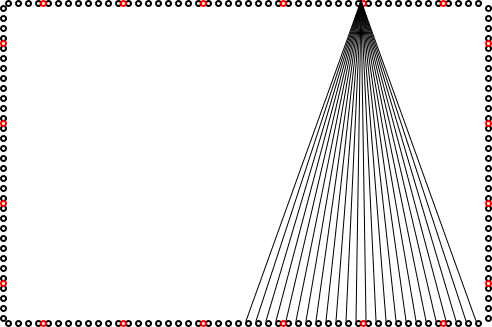
\includegraphics[width=\textwidth]{gfx/scene_rays_sample.svg}
 \centering
 \makebox[\textwidth][r]{
  \resizebox{.9\largefigure}{!}{
    \def\svgwidth{0.9\largefigure}
    \includesvg{gfx/scene_rays_sample}
  }
 }
 \caption[Wizualizacja ramki]{Wizualizacja ramki. Czarne okręgi \ppauza fotodiody; czerwone \ppauza diody LED; czarne odcinki \ppauza odbierane promienie.}
 \label{fig:scene_rays_sample}
\end{figure}

Dane o promieniach zbierane są przez mikrokontroler, opakowywane w ramki protokołu, przesyłane do komputera i po rozpakowaniu poddawane dalszemu przetwarzaniu.\\

\section{Heatmapa}

Wykorzystując te informacje można stworzyć \textit{heatmapę} prezentującą w graficzny sposób rozkład gęstości przecięć promieni zasłoniętych. Daje to możliwość wizualnego rozpoznania konturów obiektów znajdujących się wewnątrz ramki.

Wygodnym sposobem wyboru kolorów heatmapy jest wykorzystanie modelu barw HSL, przy czym wielkościom $s$ i $l$ zostały przypisane stałe wartości: $s = 1$, $l = 0.5$, natomiast parametr $h$ został dobrany w taki sposób, aby zmieniał się od $240^{\circ}$ (niebieski) do $0^{\circ}$ (czerwony) i reprezentował tym odpowiednio ,,mało'' i ,,dużo'', przy czym dokładne wartości ze skali nie mają istotnego znaczenia, a jedynie ich względna wielkość.

Heatmapa generowana jest w następujący sposób:
\begin{enumerate}
 \item Scena, wnętrze reprezentacji ramki na komputerze, dzielona jest na kwadraty $A_{x,y}$ o zadanym boku $a$, a każdemu z nich przyporządkowywany jest licznik $C$ z początkową wartością $C_{i,j} = 0$,
 \item pobierane kolejno są dane o zasłoniętych promieniach dla każdego z modułów,
 \item dla każdego zasłoniętego promienia wyznaczany jest \textit{bounding box}, z dokładnością do $a$,
 \item dla każdego kwadrata z bounding boksa promienia sprawdzane jest, czy promień przechodzi przez ten kwadrat, tj. czy przecina którąkolwiek z jego ścianek,
 \item jeśli promień przecina kwadrat $A_{i,j}$, to wartość jego licznika $C_{i,j}$ jest inkrementowana o $1$,
 \item po przetworzeniu wszystkich aktualnie dostępnych danych, znajdowana jest największa wartość licznika $C$, $C_{max}$, względem której skalowane są kolory heatmapy,
 \item dla każdego kwadrata $A_{i,j}$, jeśli $C_{i,j} > 0$, rysowany jest w scenie kwadrat o wyznaczonym kolorze.
\end{enumerate}

Wybrane kroki powyższego algorytmu prezentują rysunki \ref{fig:scene_intersections}, \ref{fig:scene_rays}, \ref{fig:scene_heatmap} oraz \ref{fig:scene_heatmap_overlay}.

\begin{sidewaysfigure}[tbh]
  \myfloatalign
  \vspace{0.085\textheight}
  \subfloat[Wizualizacja sceny wraz z jednym promieniem, bounding boksem i wybranymi przecinanymi kwadratami]
  {\label{fig:scene_intersections}
  \def\svgwidth{0.47\linewidth}
  \includesvg{gfx/scene_intersections}} \quad
  \subfloat[Wizualizacja sceny z przykładowymi promieniami]
  {\label{fig:scene_rays}%
  \def\svgwidth{0.47\linewidth}
  \includesvg{gfx/scene_rays}} \\
  \subfloat[Wizualizacja sceny z heatmapą]
  {\label{fig:scene_heatmap}
  \def\svgwidth{0.47\linewidth}
  \includesvg{gfx/scene_heatmap}} \quad
  \subfloat[Wizualizacja sceny z heatmapą i nałożonymi promieniami]
  {\label{fig:scene_heatmap_overlay}
  \def\svgwidth{0.47\linewidth}
  \includesvg{gfx/scene_heatmap_overlay}}
  \caption[Algorytm konstrukcji heatmapy]{Algorytm konstrukcji heatmapy, $a$ = 10.}\label{fig:scene_heatmap_algorithm}
\end{sidewaysfigure}

Ze względu na możliwość badania jedynie obecności lub braku promienia, system jest w stanie raportować w najlepszym przypadku otoczkę wypukłą obiektów. Otoczka wypukła zbioru punktów $A$, oznaczana zwykle $\mbox{conv} A$ to najmniejszy wypukły zbiór punktów zawierający $A$.\\

\clearpage

Na potrzeby testów i prezentacji stworzyłem dodatkową funkcjonalność pozwalającą na rozmieszczanie w scenie wirtualnych przeszkód, pozwala to przedstawić działanie algorytmów w pewnej teoretycznej, idealnej sytuacji, która nie zawsze występuje przy rozwojowym sprzęcie.

Większość przedstawianych w tym rozdziale sytuacji będzie opierać się o fikcyjne przeszkody pod postacią okręgów.\\

Wykorzystując opisany wcześniej algorytm generowania heatmapy można już zaimplementować system wykrywania przeszkód. Istotnym dla działania programu jest wybór wielkości $a$. Mniejsze wartości zwiększają rozdzielczość kosztem większej ilości danych do przetworzenia, zaś większe mogą zapewnić mniejszą podatność na szumy (fałszywe pozytywy i negatywy). Wpływ wielkości $a$ na algorytm konstruujący heatmapę prezentuje rysunek~\ref{fig:scene_heatmap_size}.

\begin{sidewaysfigure}[tbh]
  \myfloatalign
  \vspace{0.085\textheight}
  \subfloat[$a$ = 5]
  {\label{fig:scene_heatmap_5}
  \def\svgwidth{0.46\linewidth}
  \includesvg{gfx/scene_heatmap_5}} \quad
  \subfloat[$a$ = 10]
  {\label{fig:scene_heatmap_10}%
  \def\svgwidth{0.46\linewidth}
  \includesvg{gfx/scene_heatmap_10}} \\
  \subfloat[$a$ = 15]
  {\label{fig:scene_heatmap_15}
  \def\svgwidth{0.46\linewidth}
  \includesvg{gfx/scene_heatmap_15}} \quad
  \subfloat[$a$ = 20]
  {\label{fig:scene_heatmap_20}
  \def\svgwidth{0.46\linewidth}
  \includesvg{gfx/scene_heatmap_20}}
  \caption[Wpływ wielkości $a$ na algorytm konstrukcji heatmapy.]{Wpływ wielkości $a$ na algorytm konstrukcji heatmapy.}\label{fig:scene_heatmap_size}
\end{sidewaysfigure}


Jak widać, dla małych wartości $a$, miejsca przecięć promieni zakrytych wartość licznika $C$ jest niewiele większa od wartości w okolicach nadajników, gdzie zbiega się wiele promieni. Wraz ze zwiększaniem $a$ charakterystyka heatmapy zmienia się na rzecz lepszego uwidocznienia zasłaniającego obiektu, jednak maleje przy tym dostępna rozdzielczość wykrywania.\\

\section{Ulepszona heatmapa}

Problem małych wielkości licznika $C$ rozwiązałem ulepszając pierwotny algorytm generowania heatmapy wykorzystując także dane o prawdziwych negatywach, tj. promieniach, o których wiadomo, że powinny być widoczne, jeśli nie napotkały na przeszkodę.

Ulepszony algorytm wygląda następująco (zmiany zostały wyróżnione):
\begin{enumerate}
 \item Scena, wnętrze reprezentacji ramki na komputerze, dzielona jest na kwadraty $A_{x,y}$ o zadanym boku $a$, a każdemu z nich przyporządkowywany jest licznik $C$ z początkową wartością $C_{i,j} = 0$,
 \item pobierane kolejno są dane o \textit{wszystkich} promieniach dla każdego z modułów,
 \item dla \textit{każdego} uzyskanego promienia wyznaczany jest bounding box, z dokładnością do $a$,
 \item dla każdego kwadrata z bounding boksa promienia sprawdzane jest, czy promień przechodzi przez ten kwadrat, tj. czy przecina którąkolwiek z jego ścianek,
 \item jeśli \textit{zasłonięty} promień przecina kwadrat $A_{i,j}$, to wartość jego licznika $C_{i,j}$ jest inkrementowana o $1$, \textit{jeśli promień był prawdziwym negatywem, to licznik $C_{i,j}$ jest dekrementowany o $1$},
 \item po przetworzeniu wszystkich aktualnie dostępnych danych, znajdowane są \textit{ekstrema} licznika $C$: $C_{max}$ i $C_{min}$, względem których skalowane są kolory heatmapy,
 \item dla \textit{każdego} kwadrata $A_{i,j}$, rysowany jest w scenie kwadrat o wyznaczonym kolorze.\\
\end{enumerate}

Wprowadzenie tych zmian powoduje duży wzrost ilości wykonywanych obliczeń, nadal są to jednak obliczenia proste i szybkie, a także łatwo wektoryzowalne, więc małym kosztem znacząco podniosłem jakość otrzymywanych wyników.

Rezultaty ulepszonego algorytmu prezentuje rysunek~\ref{fig:scene_heatmap2_size}.

\begin{sidewaysfigure}[tbh]
  \myfloatalign
  \vspace{0.085\textheight}
  \subfloat[$a$ = 5]
  {\label{fig:scene_heatmap2_5}
  \def\svgwidth{0.46\linewidth}
  \includesvg{gfx/scene_heatmap2_5}} \quad
  \subfloat[$a$ = 10]
  {\label{fig:scene_heatmap2_10}%
  \def\svgwidth{0.46\linewidth}
  \includesvg{gfx/scene_heatmap2_10}} \\
  \subfloat[$a$ = 15]
  {\label{fig:scene_heatmap2_15}
  \def\svgwidth{0.46\linewidth}
  \includesvg{gfx/scene_heatmap2_15}} \quad
  \subfloat[$a$ = 20]
  {\label{fig:scene_heatmap2_20}
  \def\svgwidth{0.46\linewidth}
  \includesvg{gfx/scene_heatmap2_20}}
  \caption[Wpływ wielkości $a$ na ulepszony algorytm konstrukcji heatmapy.]{Wpływ wielkości $a$ na ulepszony algorytm konstrukcji heatmapy.}\label{fig:scene_heatmap2_size}
\end{sidewaysfigure}

Należy zauważyć, że chociaż obiekty zasłaniające ponownie rysowane są kolorem czerwonym, to pozostałe kolory reprezentują już inne wartości powstałe w wyniku rozciągnięcia skali w stronę liczb ujemnych.
